% Yang kami jual: tiga paket (sistem, bukan turbin) + jenjang pelanggan.
\documentclass[border=4pt]{standalone}
% Gaya bersama gambar deck Demo Day (dipakai semua gambar/*.tex standalone).
\usepackage{amssymb}
\usepackage{fontspec}
\setmainfont{DejaVu Sans Condensed}
\setsansfont{DejaVu Sans Condensed}
\newfontfamily\judulfont{DejaVu Sans}[BoldFont={DejaVu Sans Bold}, Ligatures=TeX]
\usepackage{tikz,pgfplots}
\pgfplotsset{compat=1.18, every axis/.append style={/pgf/number format/assume math mode=true, /pgf/number format/use comma, /pgf/number format/1000 sep={.}}}
\usetikzlibrary{positioning,arrows.meta,calc,shapes.geometric,fit,backgrounds}
\definecolor{gelap}{HTML}{15242B}
\definecolor{teal}{HTML}{285052}
\definecolor{amber}{HTML}{E8A317}
\definecolor{muda}{HTML}{DCE8E8}
\definecolor{abu}{HTML}{8A9499}
\definecolor{teks}{HTML}{1E2B30}
\definecolor{hijau}{HTML}{2F7D5B}
\definecolor{merah}{HTML}{A33A2A}
\color{teks}
\tikzset{
  ubin/.style={fill=muda, rounded corners=5pt, align=center, inner sep=6pt},
  inti/.style={ubin, fill=gelap, text=white},
  panah/.style={-{Stealth[length=3mm]}, line width=1.3pt, draw=amber},
  panahabu/.style={-{Stealth[length=2.5mm]}, line width=1pt, draw=abu},
  judulubin/.style={font=\judulfont\bfseries},
}
% Dibuat otomatis oleh buat_aset.py dari ml/results/energi_harian.json; jangan diedit manual.
\newcommand{\energiTurbin}{270}
\newcommand{\energiQa}{187}
\newcommand{\energiQb}{377}
\newcommand{\hariEnergi}{140}
\newcommand{\raspiWh}{71}
\newcommand{\chipWh}{4,1}
\newcommand{\raspiPersen}{26}
\newcommand{\chipPersen}{1,5}
\newcommand{\raspiPersenA}{19}
\newcommand{\raspiPersenB}{38}
\newcommand{\raspiPersenNum}{26.3}
\newcommand{\chipPersenNum}{1.5}
\newcommand{\hematKwh}{24}
\newcommand{\kaliHemat}{17}
\newcommand{\jRaspi}{182}
\newcommand{\jChip}{10,4}
\newcommand{\periodeEnergi}{2026-03-31--2026-10-20}

\AtBeginDocument{\hyphenpenalty=10000 \exhyphenpenalty=10000}

\begin{document}
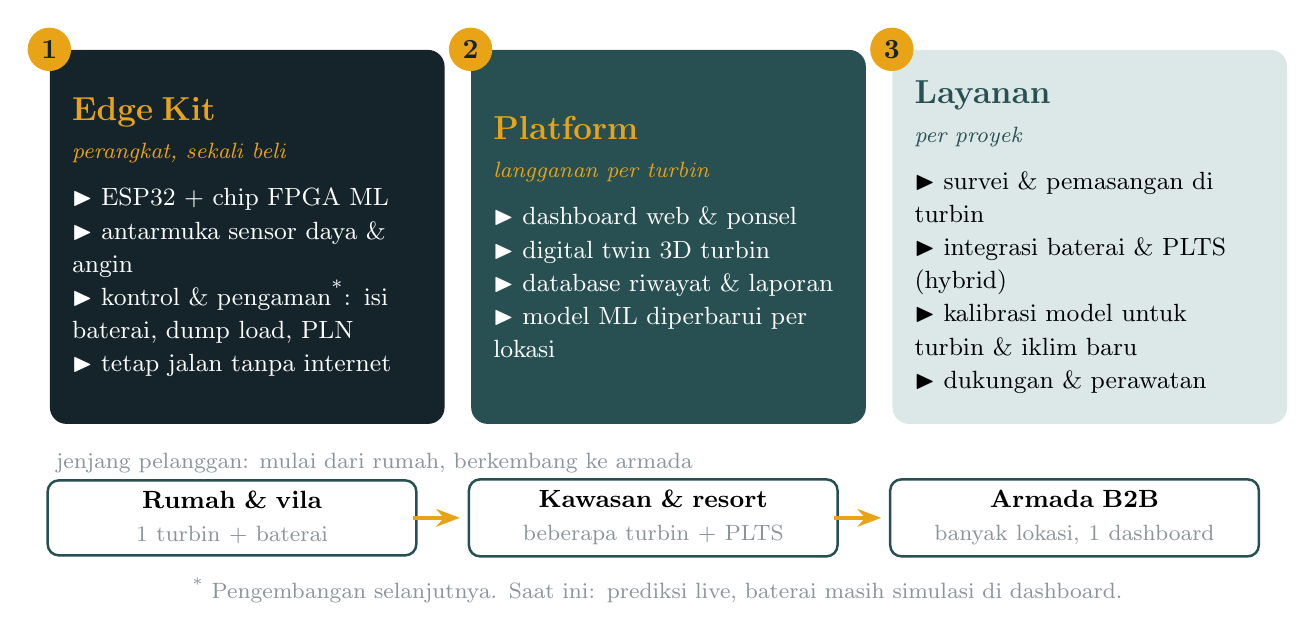
\begin{tikzpicture}[font=\fontsize{9.5}{12}\selectfont,
  kartu/.style={rounded corners=6pt, text width=4.45cm, minimum height=4.75cm, align=left, inner sep=8pt, anchor=north},
  nomor/.style={circle, fill=amber, text=gelap, font=\judulfont\bfseries, inner sep=2.5pt}]
  \def\isi#1#2#3{{\color{#3}\judulfont\bfseries\fontsize{12.5}{14}\selectfont #1}\\[2pt]{\color{#3}\fontsize{8.5}{10}\selectfont\itshape #2}\\[5pt]}
  \node[kartu, fill=gelap, text=white] (a) at (0,0) {\isi{Edge Kit}{perangkat, sekali beli}{amber}
    $\blacktriangleright$ ESP32 + chip FPGA ML\\
    $\blacktriangleright$ antarmuka sensor daya \& angin\\
    $\blacktriangleright$ kontrol \& pengaman\textsuperscript{*}: isi baterai, dump load, PLN\\
    $\blacktriangleright$ tetap jalan tanpa internet};
  \node[kartu, fill=teal, text=white] (b) at (5.35,0) {\isi{Platform}{langganan per turbin}{amber}
    $\blacktriangleright$ dashboard web \& ponsel\\
    $\blacktriangleright$ digital twin 3D turbin\\
    $\blacktriangleright$ database riwayat \& laporan\\
    $\blacktriangleright$ model ML diperbarui per lokasi};
  \node[kartu, fill=muda] (c) at (10.7,0) {\isi{Layanan}{per proyek}{teal}
    $\blacktriangleright$ survei \& pemasangan di turbin\\
    $\blacktriangleright$ integrasi baterai \& PLTS (hybrid)\\
    $\blacktriangleright$ kalibrasi model untuk turbin \& iklim baru\\
    $\blacktriangleright$ dukungan \& perawatan};
  \foreach \n/\k in {1/a,2/b,3/c} \node[nomor] at (\k.north west) {\n};
  % jenjang pelanggan
  \begin{scope}[shift={(-2.55,-5.95)}]
    \node[anchor=south west, text=abu, font=\fontsize{8.5}{10}\selectfont] at (0,0.45) {jenjang pelanggan: mulai dari rumah, berkembang ke armada};
    \foreach \x/\t/\s/\w in {0/Rumah \& vila/1 turbin + baterai/4.4, 5.35/Kawasan \& resort/beberapa turbin + PLTS/4.4, 10.7/Armada B2B/{banyak lokasi, 1 dashboard}/4.4}
      {\node[draw=teal, line width=0.9pt, rounded corners=4pt, text width=\w cm, align=center, anchor=west, inner sep=4pt] at (\x,0) {\textbf{\t}\\{\color{abu}\fontsize{8.5}{10}\selectfont\s}};}
    \draw[panah] (4.65,0) -- (5.25,0);
    \draw[panah] (10.0,0) -- (10.6,0);
  \end{scope}
  \node[anchor=north, text=abu, text width=14.6cm, align=center, font=\fontsize{8.5}{10}\selectfont] at ([yshift=-4pt]current bounding box.south) {\textsuperscript{*} Pengembangan selanjutnya. Saat ini: prediksi live, baterai masih simulasi di dashboard.};
\end{tikzpicture}
\end{document}
